\documentclass[12pt, a4paper]{article}
\usepackage{../../../myconfig} % Gọi file cấu hình từ ngoài gốc vào

% ==========================================
% BẮT ĐẦU NỘI DUNG TÀI LIỆU
% ==========================================
\begin{document}

% Truyền 3 tham số: {Nhãn cam} {Chữ to chính giữa} {Chữ ở góc phải Header}
\titlebox{Chủ đề: Thống kê}{Các số đặc trưng đó phân tán - ghép nhóm}{Thống kê - ghép nhóm}

% --- CÂU 1 ---
\questionLinesManual{0}{1}{Công ty X muốn khảo sát mức chi phí thuê nhà hàng tháng của các nhân viên độc thân để có chính sách hỗ trợ phù hợp. Một nhóm nghiên cứu đã thu thập dữ liệu từ 100 nhân viên độc thân về số tiền họ phải chi trả cho việc thuê nhà hàng tháng (đơn vị: triệu đồng) ở bảng dưới đây:

\begin{center}
\begin{tabular}{|c|c|c|c|c|c|c|}
\hline
Tiền thuê nhà (triệu đồng) & \([1;2)\) & \([2;3)\) & \([3;4)\) & \([4;5)\) & \([5;6)\) & \([6;7)\) \\
\hline
Số nhân viên & 17 & 28 & 24 & 15 & 9 & 7 \\
\hline
\end{tabular}
\end{center}

Tính độ lệch chuẩn của mẫu số liệu ghép nhóm về chi phí thuê nhà hàng tháng của các nhân viên độc thân ở công ty X (kết quả làm tròn đến hàng phần trăm).}{%
    \begin{tasks}(4)
        \task 2,1
        \task 1,45
        \task 2,09
        \task 1,44
    \end{tasks}
}



% --- CÂU 2 ---
\questionLinesManual{0}{2}{Một giống cây xoan đào được trồng tại địa điểm X. Người ta thống kê đường kính thân của một số cây xoan đào 7 năm tuổi (đơn vị: cm) ở biểu đồ sau:

\begin{center}
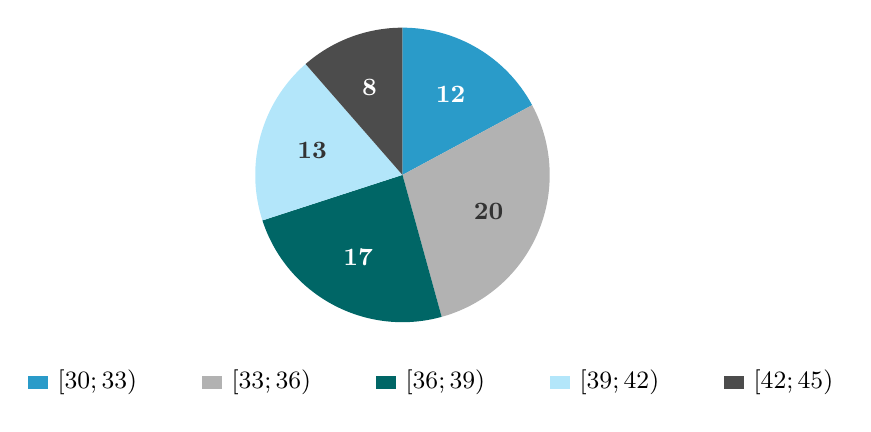
\begin{tikzpicture}[scale=0.85]

    % Nhóm [30;33) - Màu xanh lam lá
    \fill[cyan!80!black] (0,0) -- (90:2.2) arc (90:28.29:2.2) -- cycle;
    \node[white, font=\bfseries\small] at (59.14:1.4) {12};

    % Nhóm [33;36) - Màu xám
    \fill[gray!60] (0,0) -- (28.29:2.2) arc (28.29:-74.57:2.2) -- cycle;
    \node[black!80, font=\bfseries\small] at (-23.14:1.4) {20};

    % Nhóm [36;39) - Màu xanh ngọc đậm
    \fill[teal!80!black] (0,0) -- (-74.57:2.2) arc (-74.57:-162.0:2.2) -- cycle;
    \node[white, font=\bfseries\small] at (-118.28:1.4) {17};

    % Nhóm [39;42) - Màu xanh nhạt
    \fill[cyan!30] (0,0) -- (-162.0:2.2) arc (-162.0:-228.86:2.2) -- cycle;
    \node[black!80, font=\bfseries\small] at (-195.43:1.4) {13};

    % Nhóm [42;45) - Màu xám đậm
    \fill[black!70] (0,0) -- (-228.86:2.2) arc (-228.86:-270:2.2) -- cycle;
    \node[white, font=\bfseries\small] at (-249.43:1.4) {8};

    % Chú thích (Chú giải phía dưới)
    \begin{scope}[yshift=-3.2cm, xshift=-4cm, font=\small]
        \fill[cyan!80!black] (-1.6,0) rectangle (-1.3,0.2);
        \node[right] at (-1.3,0.1) {$[30;33)$};

        \fill[gray!60] (1,0) rectangle (1.3,0.2);
        \node[right] at (1.3,0.1) {$[33;36)$};

        \fill[teal!80!black] (3.6,0) rectangle (3.9,0.2);
        \node[right] at (3.9,0.1) {$[36;39)$};

        \fill[cyan!30] (6.2,0) rectangle (6.5,0.2);
        \node[right] at (6.5,0.1) {$[39;42)$};

        \fill[black!70] (8.8,0) rectangle (9.1,0.2);
        \node[right] at (9.1,0.1) {$[42;45)$};
    \end{scope}
\end{tikzpicture}
\end{center}

Khoảng tứ phân vị của mẫu số liệu ghép nhóm trên gần bằng}{%
    \begin{tasks}(4)
        \task 5,98
        \task 5,96
        \task 5,99
        \task 5,97
    \end{tasks}
}





\noindent\textbf{Dùng dữ kiện sau để trả lời các câu 03, 04 phía dưới}

\vspace{0.2cm}

\noindent Anh T đầu tư số tiền bằng nhau vào hai lĩnh vực kinh doanh $M$ và $N$. Sau 60 tháng, anh thống kê số tiền thu được hàng tháng (đơn vị: \textit{triệu đồng}) từ mỗi lĩnh vực để đánh giá hiệu quả đầu tư và thu được kết quả sau:

\begin{figure}[htbp]
\centering
\begin{tikzpicture}[scale=1, >=stealth]
    % Định nghĩa màu sắc cho 2 lĩnh vực
    \definecolor{colorM}{RGB}{0, 140, 160} % Màu xanh lá/lam (Lĩnh vực M)
    \definecolor{colorN}{RGB}{128, 128, 128} % Màu xám (Lĩnh vực N)

    % 1. Đường lưới ngang và trục Oy
    \foreach \y in {0, 5, 10, 15, 20, 25, 30} {
        \draw[gray!30, thin] (0, \y*0.18) -- (12, \y*0.18);
        \node[left, font=\small] at (0, \y*0.18) {\y};
    }

    % Macro vẽ cột dữ liệu
    % \drawbar{x_pos}{height}{color}{label}
    \newcommand{\drawbar}[4]{
        \fill[#3] (#1, 0) rectangle (#1 + 0.5, #2*0.18);
        \node[above, font=\small] at (#1 + 0.25, #2*0.18) {#4};
    }

    % Nhóm [5; 10)
    \drawbar{0.8}{18}{colorM}{18}
    \drawbar{1.35}{4}{colorN}{4}

    % Nhóm [10; 15)
    \drawbar{3.1}{7}{colorM}{7}
    \drawbar{3.65}{15}{colorN}{15}

    % Nhóm [15; 20)
    \drawbar{5.4}{12}{colorM}{12}
    \drawbar{5.95}{24}{colorN}{24}

    % Nhóm [20; 25)
    \drawbar{7.7}{9}{colorM}{9}
    \drawbar{8.25}{10}{colorN}{10}

    % Nhóm [25; 30)
    \drawbar{10.0}{14}{colorM}{14}
    \drawbar{10.55}{7}{colorN}{7}

    % 2. Trục tọa độ và Nhãn trục Ox, Oy
    \draw[gray!60, thick] (0,0) -- (12.2,0);
    \draw[gray!60, thick] (0,0) -- (0,5.6);

    \node[below, font=\small] at (1.325, -0.1) {$[5; 10)$};
    \node[below, font=\small] at (3.625, -0.1) {$[10; 15)$};
    \node[below, font=\small] at (5.925, -0.1) {$[15; 20)$};
    \node[below, font=\small] at (8.225, -0.1) {$[20; 25)$};
    \node[below, font=\small] at (10.525, -0.1) {$[25; 30)$};

    \node[rotate=90, font=\small] at (-0.9, 2.7) {Số tháng};
    \node[font=\small] at (6.125, -1.2) {Triệu đồng};

    % 3. Tiêu đề
    \node[align=center, font=\bfseries] at (6.125, 6.0) {Số tiền thu được hàng tháng từ hai lĩnh vực kinh doanh M và N};

    % 4. Chú thích (Legend)
    \begin{scope}[yshift=-1.4cm, xshift=1.8cm, font=\small]
        \fill[colorM] (-2.35,-1) rectangle (-2, -0.8);
        \node[right] at (-2, -0.9) {Số tháng đầu tư vào lĩnh vực M};

        \fill[colorN] (5.0,-1) rectangle (5.35, -0.8);
        \node[right] at (5.35, -0.9) {Số tháng đầu tư vào lĩnh vực N};
    \end{scope}

\end{tikzpicture}
\end{figure}

% --- CÂU 3 ---
\questionLinesManual{0}{3}{Phương sai của mẫu số liệu ghép nhóm về số tiền thu được hàng tháng từ lĩnh vực kinh doanh N gần nhất với giá trị nào dưới đây?}{%
    \begin{tasks}(4)
        \task 59,7
        \task 59,8
        \task 28,7
        \task 28,8
    \end{tasks}
}

% --- CÂU 4 ---
\questionLinesManual{0}{4}{Nếu so sánh theo độ lệch chuẩn thì độ rủi ro của lĩnh vực kinh doanh M cao hơn lĩnh vực kinh doanh N bao nhiêu? (kết quả làm tròn đến chữ số thập phân thứ hai)}{%
    \begin{tasks}(4)
        \task 2,34
        \task 2,35
        \task 2,36
        \task 2,37
    \end{tasks}
}


% --- CÂU 12 ---
\questionLinesManual{0}{5}{Một trung tâm mua sắm đã thống kê lại hóa đơn (tính bằng triệu đồng) của các khách hàng trong một ngày ở bảng sau:

\begin{center}
\begin{tabular}{|c|c|c|c|c|c|c|}
\hline
Hóa đơn & \([0;0,5)\) & \([0,5;1)\) & \([1;1,5)\) & \([1,5;2)\) & \([2;2,5)\) & \([2,5;3)\) \\
\hline
Số hóa đơn & 13 & 35 & 27 & 14 & 8 & 3 \\
\hline
\end{tabular}
\end{center}

Tứ phân vị thứ nhất của mẫu số liệu ghép nhóm về hóa đơn của các khách hàng trong một ngày gần bằng bao nhiêu? (Kết quả làm tròn đến hàng phần trăm).
}
{%
    \begin{tasks}(4)
        \task 0.67
        \task 0.57
        \task 0.72
        \task 0.81
    \end{tasks}
}



% --- CÂU 9 ---
\questionTrueFalse{0}{6}{Kết quả thống kê về điểm trung bình năm học của học sinh hai lớp 12A và 12B được biểu diễn trong bảng dưới đây:

\begin{center}
\begin{tabular}{|c|c|c|c|c|c|}
\hline
Điểm trung bình & \([5;6)\) & \([6;7)\) & \([7;8)\) & \([8;9)\) & \([9;10)\) \\
\hline
Số học sinh lớp 12A & 4 & 15 & 20 & 9 & 2 \\
\hline
Số học sinh lớp 12B & 6 & 14 & 22 & 7 & 1 \\
\hline
\end{tabular}
\end{center}
}{
    \textbf{a)} & Phương sai của mẫu số liệu ghép nhóm về điểm trung bình năm học của học sinh lớp 12A bằng 0,92.
    & \textcolor{amberorange}{$\bigcirc$} & \textcolor{amberorange}{$\bigcirc$} \\ \hline
    
    \textbf{b)} & Khoảng tứ phân vị của mẫu số liệu ghép nhóm về điểm trung bình năm học của học sinh lớp 12B gần bằng 1,33.
    & \textcolor{amberorange}{$\bigcirc$} & \textcolor{amberorange}{$\bigcirc$} \\ \hline
    
    \textbf{c)} & Nếu so sánh theo độ lệch chuẩn của mẫu số liệu ghép nhóm thì học sinh lớp 12A có điểm trung bình đồng đều hơn lớp 12B.
    & \textcolor{amberorange}{$\bigcirc$} & \textcolor{amberorange}{$\bigcirc$} \\ \hline
    
    \textbf{d)} & Nếu so sánh theo khoảng tứ phân vị của mẫu số liệu ghép nhóm thì học sinh lớp 12B có điểm trung bình đồng đều hơn lớp 12A.
    & \textcolor{amberorange}{$\bigcirc$} & \textcolor{amberorange}{$\bigcirc$} \\
}

% --- CÂU 8 ---
\questionTrueFalse{0}{7}{Chỉ số ô nhiễm không khí (AQI) tại thủ đô Hà Nội trong tháng 6/2024 được thống kê vào 10h30 sáng các ngày trong tháng được thể hiện trong bảng sau:

\begin{center}
\begin{tabular}{|c|c|c|c|c|c|}
\hline
Chỉ số & \([130;145)\) & \([145;160)\) & \([160;175)\) & \([175;190)\) & \([190;205)\) \\
\hline
Số ngày & 8 & 7 & 6 & 7 & 2 \\
\hline
\end{tabular}
\end{center}
}{
    \textbf{a)} & Chỉ số ô nhiễm không khí trung bình tại thủ đô Hà Nội trong tháng 6/2024 bằng 161.
    & \textcolor{amberorange}{$\bigcirc$} & \textcolor{amberorange}{$\bigcirc$} \\ \hline
    
    \textbf{b)} & Khoảng biến thiên của mẫu số liệu ghép nhóm về chỉ số ô nhiễm không khí tại thủ đô Hà Nội trong tháng 6/2024 bằng 60.
    & \textcolor{amberorange}{$\bigcirc$} & \textcolor{amberorange}{$\bigcirc$} \\ \hline
    
    \textbf{c)} & Tứ phân vị thứ ba của mẫu số liệu ghép nhóm về chỉ số ô nhiễm không khí tại thủ đô Hà Nội trong tháng 6/2024 gần bằng 178,2.
    & \textcolor{amberorange}{$\bigcirc$} & \textcolor{amberorange}{$\bigcirc$} \\ \hline
    
    \textbf{d)} & Khoảng tứ phân vị của mẫu số liệu ghép nhóm về chỉ số ô nhiễm không khí tại thủ đô Hà Nội trong tháng 6/2024 gần bằng 34,15.
    & \textcolor{amberorange}{$\bigcirc$} & \textcolor{amberorange}{$\bigcirc$} \\
}



% --- CÂU 11 ---
\questionShortAnswer{0}{8}{Thầy Minh thống kê điểm thi khảo sát chất lượng môn Toán của học sinh lớp 12D thu được mẫu số liệu ghép nhóm sau:

\begin{center}
\begin{tabular}{|c|c|c|c|c|c|}
\hline
Điểm thi & \([0;2)\) & \([2;4)\) & \([4;6)\) & \([6;8)\) & \([8;10)\) \\
\hline
Số học sinh & 0 & 3 & 9 & 16 & 2 \\
\hline
\end{tabular}
\end{center}

Khoảng biến thiên của mẫu số liệu ghép nhóm về điểm thi khảo sát chất lượng môn Toán của học sinh lớp 12D bằng bao nhiêu?
}

% --- CÂU 13 ---
\questionShortAnswer{0}{9}{Một hãng xe ô tô thống kê lại số lần gặp sự cố về động cơ của 100 chiếc xe cùng loại sau 3 năm sử dụng đầu tiên ở bảng sau:

\begin{center}
\begin{tabular}{|c|c|c|c|c|c|}
\hline
Số lần gặp sự cố & \([0,5;2,5)\) & \([2,5;4,5)\) & \([4,5;6,5)\) & \([6,5;8,5)\) & \([8,5;10,5)\) \\
\hline
Số xe & 18 & 32 & 26 & 20 & 4 \\
\hline
\end{tabular}
\end{center}

Tìm khoảng tứ phân vị của mẫu số liệu ghép nhóm về số lần gặp sự cố về động cơ của 100 chiếc xe cùng loại sau 3 năm sử dụng đầu tiên. (Kết quả làm tròn đến chữ số hàng phần trăm).
}


% --- CÂU 13 ---
\questionShortAnswer{0}{10}{Để đánh giá mức độ cân bằng giữa học tập và công việc làm thêm của sinh viên, ban quản lý của trường đại học X đã thực hiện một cuộc khảo sát về số giờ làm thêm mỗi tuần của sinh viên trong trường. Dữ liệu được tổng hợp trong bảng sau:

\begin{center}
\begin{tabular}{|c|c|c|c|c|c|}
\hline
Số giờ làm thêm (giờ) & \([2;4)\) & \([4;6)\) & \([6;8)\) & \([8;10)\) & \([10;12)\) \\
\hline
Số sinh viên & 10 & 23 & 35 & 20 & 12 \\
\hline
\end{tabular}
\end{center}

Hãy tính độ lệch chuẩn của mẫu số liệu ghép nhóm trên (làm tròn đến hàng phần trăm) để xem mức độ chênh lệch thời gian làm thêm giữa các sinh viên.
}



\end{document}